\chapter{Results}\label{chapter:results}
%Tables
%charts
\section{Sample applications made using the framework}

\section{Benchmarks}
\label{sec:benchmarks}
  The benchmark results illustrated in this chapter were performed on Amazon EC2 server\footnote{EC2 servers of Frankfurt data center} with configurations shown in table~\autoref{tab:specs}

\begin{table}[htsb]
  \caption[Specification of machines used for testing and benchmarking]{Specification of machines used for testing and benchmarking}\label{tab:specs}
  \centering
  \begin{tabular}{l l l}
    \toprule
      Deployed Systems & Name &  Specifications\\
    \midrule

      \pbox{30cm}{\relax RabbitMQ and\\a Message Queuing System} & c3.2xLarge & \pbox{60cm}{8 core CPU, 28 ECU,\\15 GiB Memory, SSD disk}\\
\midrule
      \pbox{30cm}{\relax Message Queuing System} & m3.2xLarge & \pbox{60cm}{8 core CPU, 26 ECU,\\30 GiB Memory, SSD disk}\\
\midrule
      \pbox{20cm}{\relax Registry and\\File Server} & m3.xLarge & \pbox{60cm}{2 core CPU, 13 ECU,\\15 GiB Memory, SSD disk}\\
\midrule
      \pbox{20cm}{\relax Isolate Systems (Nodes)} & m3.xLarge & \pbox{60cm}{2 core CPU, 13 ECU,\\15 GiB Memory, SSD disk}\\

    \bottomrule
  \end{tabular}
\end{table}

\subsection{Prefetch Count}
\label{subsec:prefetchCount}
\autoref{fig:result-prefetch} shows the variation in overall message consumption when the number of consumers (separate isolate systems in separate nodes) were increased. Each line in the figure represents different values of prefetch-count set in the consumer while subscribing to the message broker system. Depending upon prefetch-count, saturation point and decrease rate can also be seen when number of consumers were increased.

  The increase in consumers had significant positive result for message throughput, but we can see that after around 8 consumers, adding more consumers had negative effect in the overall throughput.

    Increasing prefetch count had more positive impact in message throughput compared to increasing consumers. For instance, increase in consumers from 1 to 16 resulted in the rise of approximately 2000 message per second, while the increase in prefetch count from 1 to 16 in single consumer resulted in increase of message throughput by approximately 5500 messages per second.

\begin{figure}[H]
  \centering
  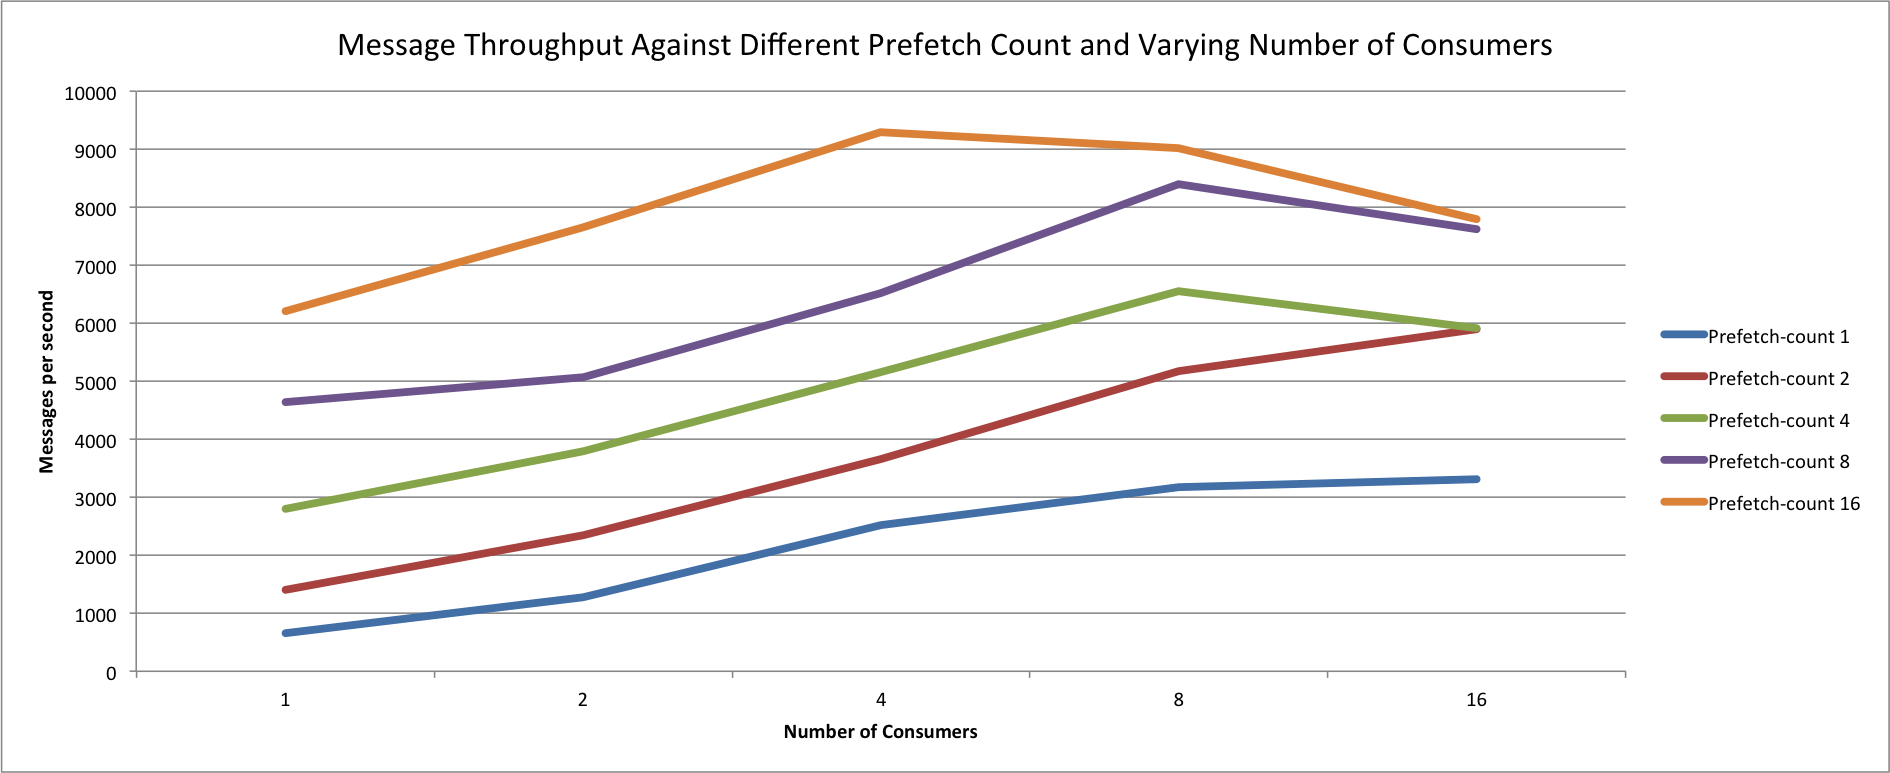
\includegraphics[width=1\textwidth]{figures/01prefetch}
  \caption[Message Throughput vs Number of consumers for varying prefetch-count]{Message Throughput vs Number of consumers for varying prefetch-count (Higher is better)}
  \label{fig:result-prefetch}
\end{figure}

\subsection{Message Size}
\label{subsec:messageSize}
The result shown in \autoref{fig:result-consumptionMessageSize} was obtained by allowing eight consumers with the prefetch count of 8 to dequeue existing messages from a queue.

  The negative effect, on message consumption throughput, of larger message is evident from the  \autoref{fig:result-consumptionMessageSize}. The decrease in message throughput was more prominent between message size of 256 bytes and 512 bytes than that of between 64 bytes and 256 bytes.

  Similar observation can be made from~\autoref{fig:result-productionMessageSize} which is a result of allowing a single worker isolate to create messages, except there was a slight rise in the throughput when the message size was increase from 512 bytes to 1024 bytes.

\begin{figure}[H]
  \centering  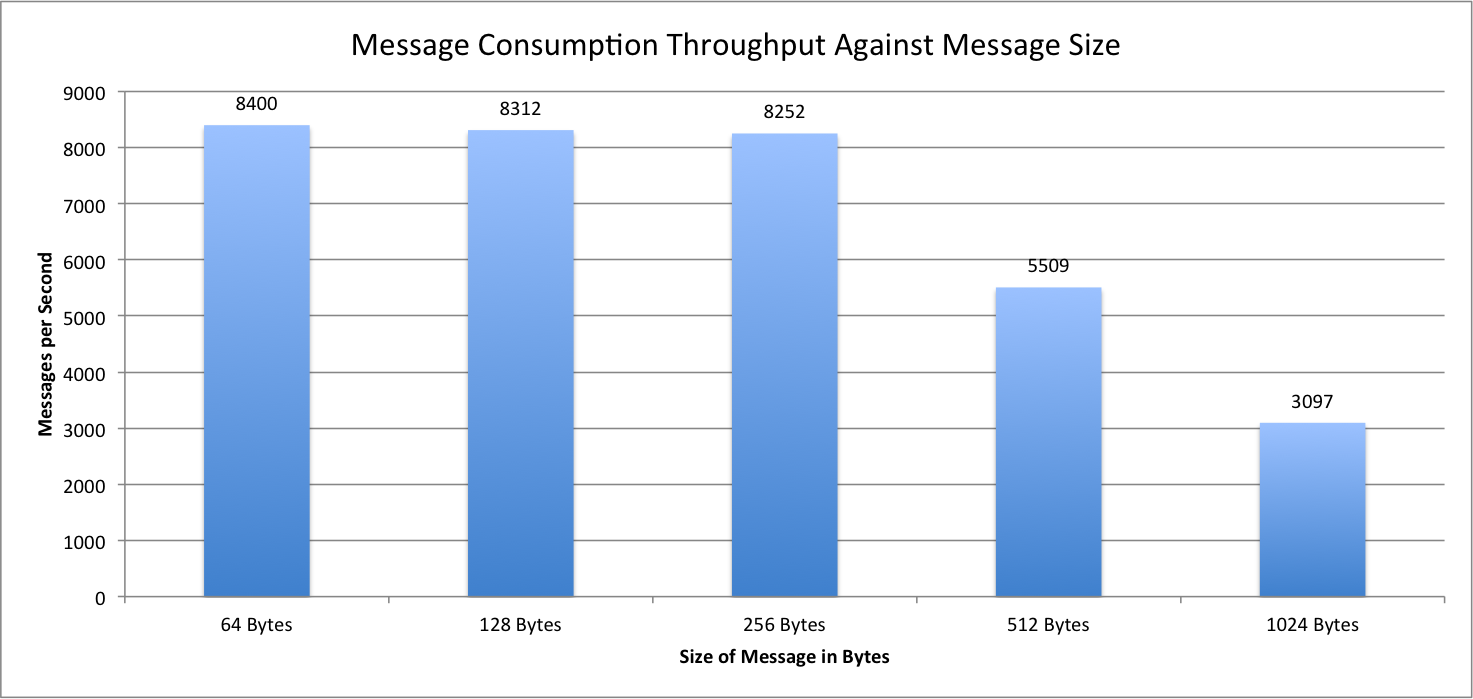
\includegraphics[width=1\textwidth]{figures/02consumptionMessageSize}
  \caption[Message Consumption Throughput vs Message Size]{Message Consumption Throughput vs Message Size (Higher is better)}
  \label{fig:result-consumptionMessageSize}
\end{figure}

\begin{figure}[H]
  \centering  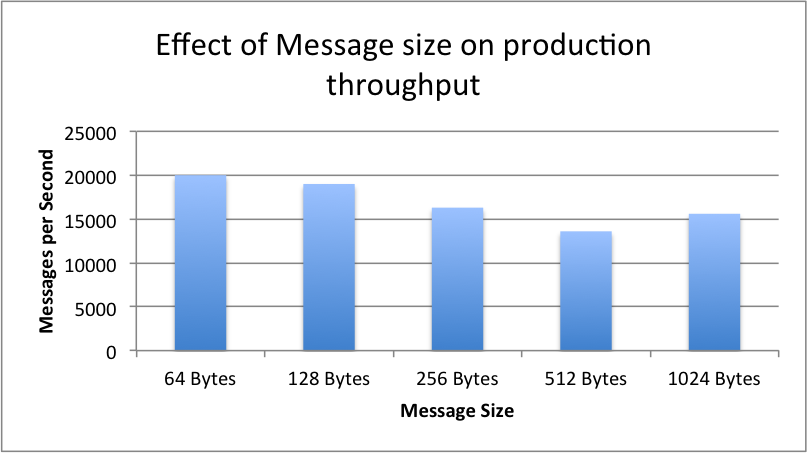
\includegraphics[width=0.8\textwidth]{figures/03productionMessageSize}
  \caption[Message Production Throughput vs Message Size]{Message Production Throughput vs Message Size (Higher is better)}
  \label{fig:result-productionMessageSize}
\end{figure}

\subsection{Number of Message Queuing Systems}
  The \autoref{fig:result-varyingMqs} is the result obtained by testing message consumption by consumers ranging from 1 to 32 distributed to one to four MQS instances connected to same instance of message broker. Multiple parallel instances of MQS clearly had better message throughput than having a single instance of MQS. Nevertheless, adding more than eight consumers per MQS instance had negative effect, as we can see from the fall of throughputs in the line chart of single MQS and that of two MQS. In the tests with one and two MQS the optimum performance was seen when there were 8 consumers in total, but with four MQS, the throughput kept rising and supported upto 32 consumers without fall in the performance. Nevertheless, the rate of performance increase was not as much as the rate seen when scaling up from two MQS to four MQS.

  The positive impact of scaling out MQS was seen not only on consumption throughput but also on production throughput. \autoref{fig:result-productionRabbit} shows the result of message production throughput by increasing number of producers from one to eight distributed among multiple instances of instances of MQS. The production rate measured here was the rate at which RabbitMQ enqueued the messages, not the rate at which a worker isolate produced messages.
\begin{figure}[H]
  \centering
  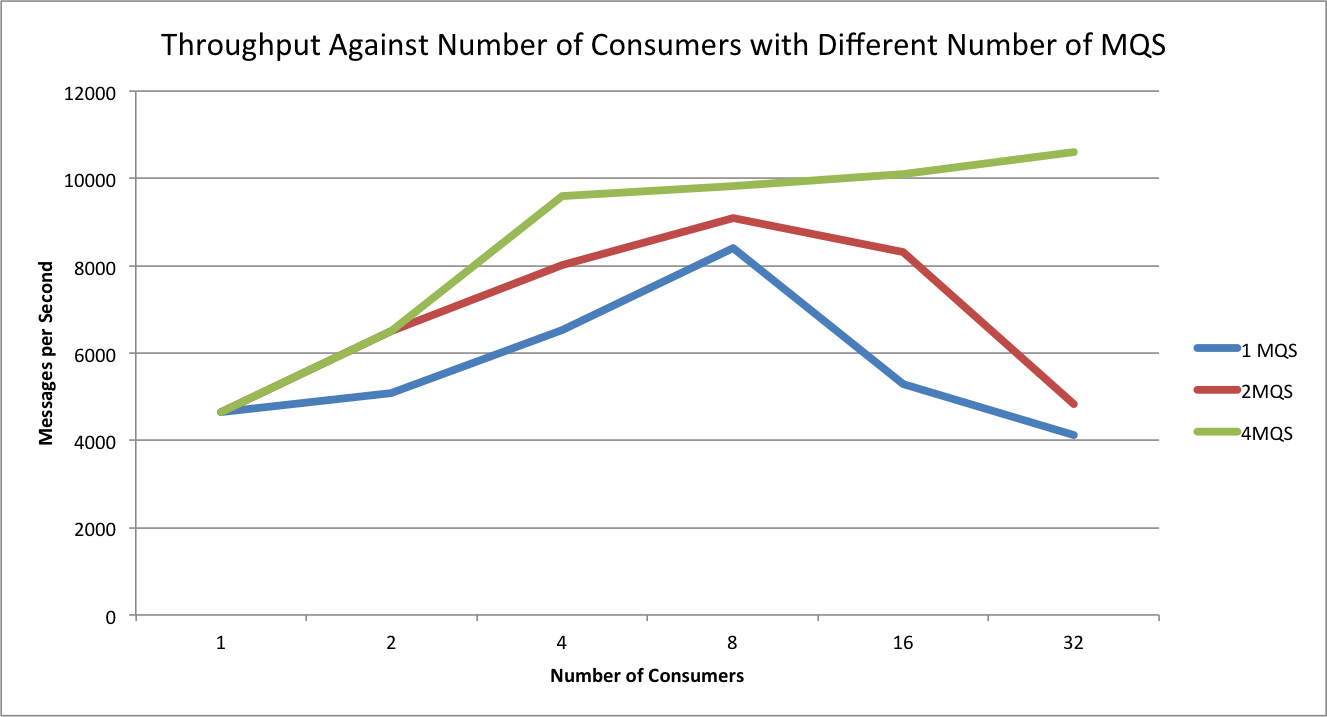
\includegraphics[width=1\textwidth]{figures/04varyingMqs}
  \caption[Consumption Throughput on Scaled out Message Queuing System]{Consumption Throughput on Scaled out Message Queuing System}
  \label{fig:result-varyingMqs}
\end{figure}


\begin{figure}[H]
  \centering  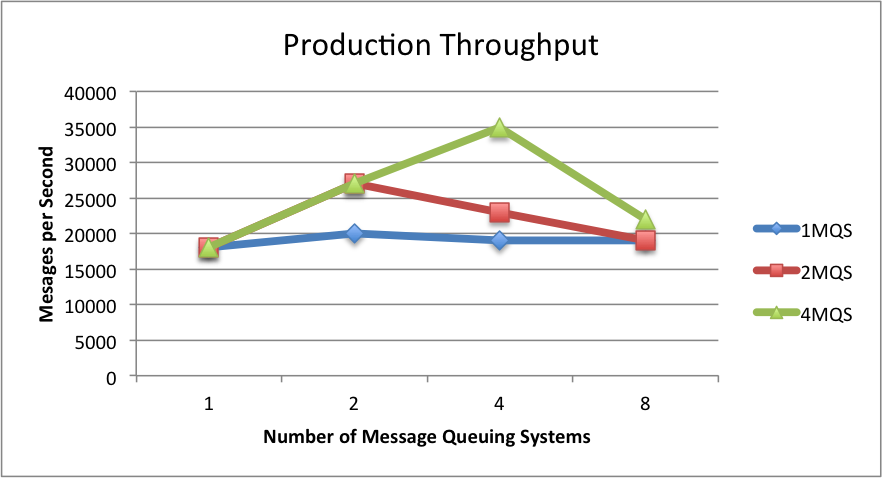
\includegraphics[width=0.9\textwidth]{figures/05productionRabbit}
  \caption[Production Throughput on Scaling out Message Queuing System]{Production Throughput on Scaling out Message Queuing System}
  \label{fig:result-productionRabbit}
\end{figure}


\subsection{Production Throughput of Isolates}
  In contrast to results of production throughput of messages in other measurements as seen on \autoref{fig:result-productionMessageSize} and \autoref{fig:result-productionRabbit}, the result shown in
 \autoref{fig:result-productionIsolate} measures the throughput of message production by the isolate system before it is sent to Message Queuing System and to Message Broker System for enqueuing. The production of a message in Worker isolate was throttled, so that there is no immediate ‘out of memory’ error by overwhelming production of messages. The message production was throttled by delaying the production of messages by random amount of time ranging from 20 micro seconds to 500 micro seconds. The observations made here are the average throughput of each worker isolate as well as average throughput of all the producer nodes connecting to single instance of MQS.

  As observed in the \autoref{fig:result-productionIsolate}, the total production rate of the messages sharply increased with increase in number of producer nodes. In contrast, the average production of single node was seen lower with higher number of producers.

  In Dart version 1.7.2, time required to send a message of ‘Map’ datatype from one isolate to another consumed around 300-500 microseconds. But, when the same message was serialized to JSON String the time required to send a message dropped to 10 - 40 microseconds. It is an improvement in speed by the factor of 10.

\begin{figure}[H]
  \centering
  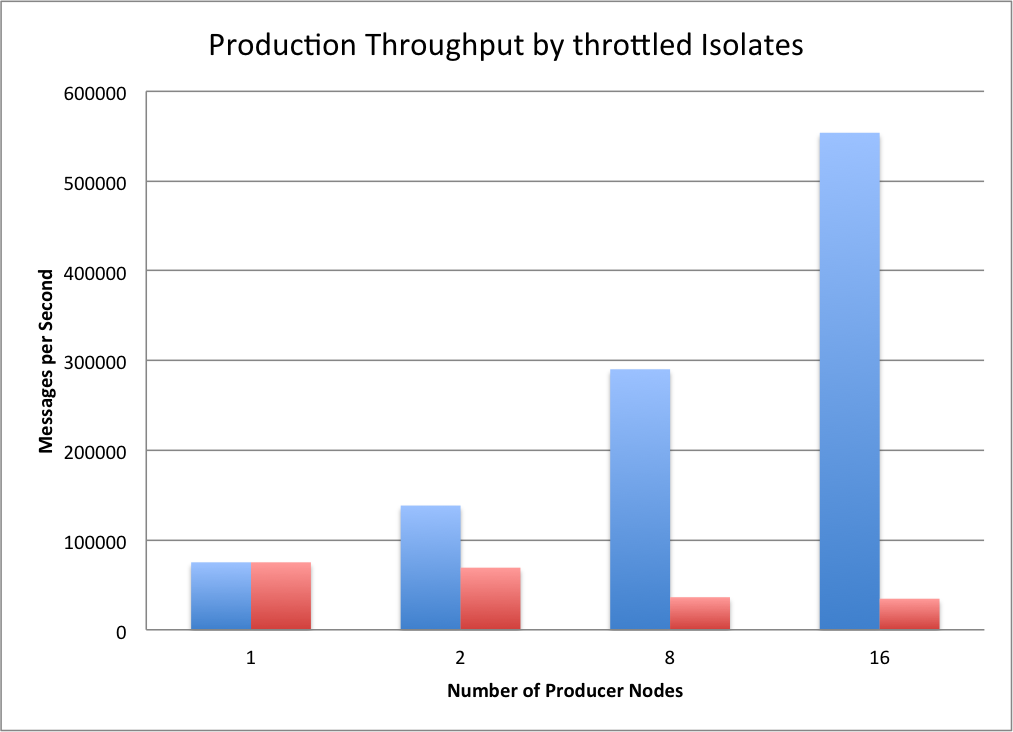
\includegraphics[width=1\textwidth]{figures/06productionIsolate}
  \caption[Production Throughput of Isolate]{Production Throughput of Isolate}
  \label{fig:result-productionIsolate}
\end{figure}

\subsection{Simultaneous Production and Consumption}
\label{subsec:simultaneous}
  In contrast to previous benchmarks, which were measured with either only producers or only consumers, the benchmarks \autoref{fig:result-simultaneous1} and \autoref{fig:result-simultaneous2} shows the consumption rate and production rate of messages when they are run simultaneously but in different nodes. Compared to what were seen on \autoref{fig:result-prefetch} and
  \autoref{fig:result-varyingMqs}, the consumption rate is lower in this case. Nevertheless, the production rate of messages remained almost equal to that was observed in \autoref{fig:result-varyingMqs} with single MQS.

  If we compare the \autoref{fig:result-simultaneous1} and \autoref{fig:result-simultaneous2}, the scaling out of MQS with producers in one MQS and consumers in another had significant positive impact in overall message throughput. Especially, in this case the consumption rate increased by almost ten times than that of using single MQS. A slight increase in production throughput was also observed with the additional MQS.

\begin{figure}[H]
  \centering
  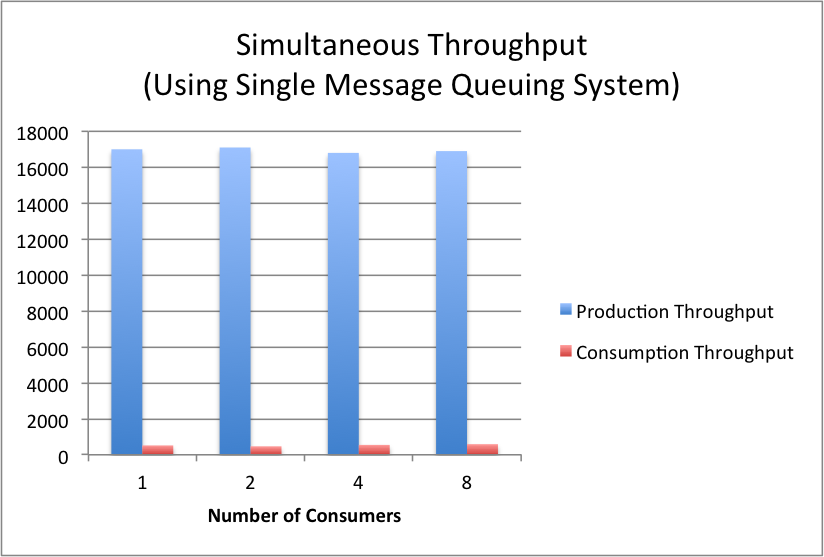
\includegraphics[width=0.8\textwidth]{figures/07simultaneous1}
  \caption[Throughput during simultaneous execution in single MQS]{Throughput during simultaneous execution in single MQS}
  \label{fig:result-simultaneous1}
\end{figure}

\begin{figure}[H]
  \centering
  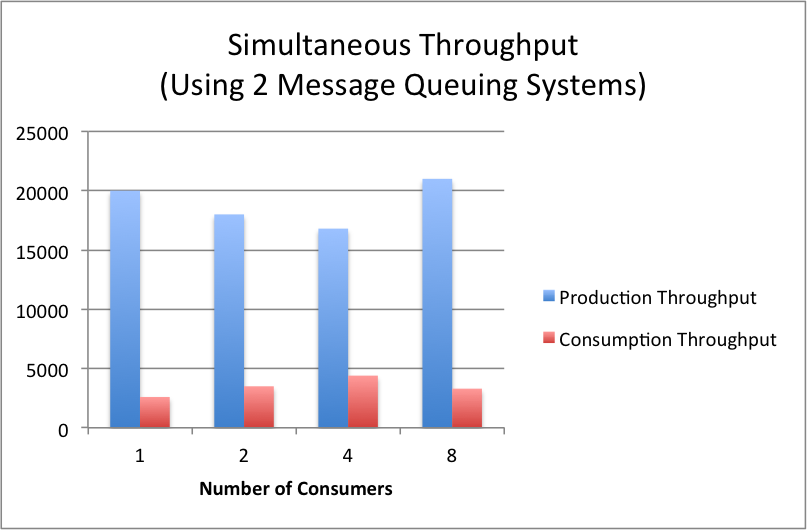
\includegraphics[width=0.8\textwidth]{figures/08simultaneous2}
  \caption[Throughput during simultaneous execution in two MQS]{Throughput during simultaneous execution in two MQS}
  \label{fig:result-simultaneous2}
\end{figure}


\subsection{Throughput of Request-Reply}
\label{subsec:request-reply}
  The request-reply application used for testing is different from producer-consumer application in terms of how the messages are produced and consumed. In request-reply, a message is produced by the producer only when it receives a request from the requester (and the requester sends request for another message only after it receives the reply) whereas, in producer-consumer application the producer creates messages regardless of existence of consumer. Also, in producer-consumer application any instance of target worker isolate of any node may consume the message as it is designated only by the name of the worker isolate. But, in request-reply the produced message is replied exactly to the same instance of the worker isolate system which sent the request message.

  For single execution of a message in producer-consumer, the steps required are enqueuing the message from producer and then dequeuing the message by the consumer. Whereas, in case of request-reply, first a request message has to be enqueued and dequeued, as a reply of which, another message will be enqueued and dequeued. Thus, the steps required in request-reply is twice as much as steps required in the producer-consumer case.

  From \autoref{fig:result-request-reply}, when the number of consumers were increased we can see the linear increment in the production and consumption rate of message. However, adding more suppliers had very little effect in overall throughput. The maximum rise in the throughput by adding suppliers was seen when there were more number of consumers.
\begin{figure}[H]
  \centering
  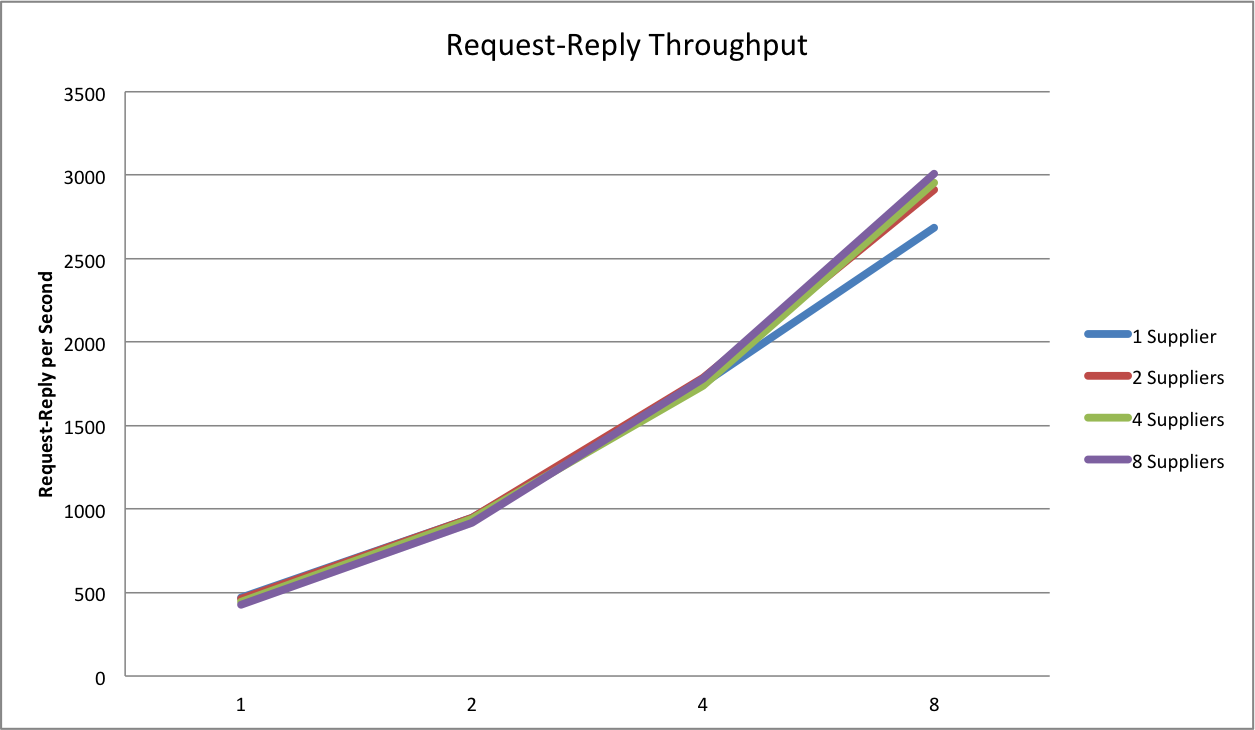
\includegraphics[width=0.85\textwidth]{figures/09request-reply}
  \caption[Throughput of request-reply]{Throughput of request-reply}
  \label{fig:result-request-reply}
\end{figure}
